
\chapter{Category Theory}


\section{Introducing Category Theory I}

A \textit{category} is a special kind of graph. Recall from Discrete mathematics, 
the formal definition of a directed graph. 


We now directed graph graphs to be \textit{labelled} directed graphs. 
We give a formal definition for a \textit{labelled} directed graphs. 

\highlightdef{A \textbf{Labelled Directed Graph} is a tuple 
$\langle N, L, s, t \rangle$ where... }

\begin{itemize}   
\renewcommand{\labelitemi}{$\Box$}
\item \textbf{Node Set} $N$ is a set of nodes
\item \textbf{Edge Set} $E$ is a set of nodes 
\item \textbf{Edge Source Function} $s:E \rightarrow N$ is a \textit{source function} 
that given an edge, outputs the source node of that edge.
\item \textbf{Edge Target Function} $t:E \rightarrow N$ is a \textit{target function}
that given an edge, outputs the target node of that edge.
\end{itemize}

Note that the source function and target function are total functions. 
Every edge has exactly one source and exactly one target. 

\begin{example}
For the following graph, using the formal definition, 
state the values of $\langle N, L, s, t \rangle$. 




\end{example}

\begin{example}
For the following graph, using the formal definition, 
state the values of $\langle N, L, s, t \rangle$. 
\end{example}

\begin{example}
For the following graph, using the formal definition, 
state the values of $\langle N, L, s, t \rangle$. 
\end{example}

The previous example highlights an important point. 
Notice that under this definition, our graph's do not have to be simple.
Given two nodes $A$ and $B$, there can be multiple edges from $A$ to $B$. 
This is not true for typical definitions of 
directed graphs (like this one we gave at the start).  

Also, note that every unlabelled direct graph can be 
transformed into a labelled graph 
where each edge $(A,B)$ is given the label $(A,B)$.


\highlightdef{A \textbf{Category} is a labelled graph with \textit{composite edges}
and \textit{identity edges} that satisfy \textit{algebraic laws}}

Formally, a category is a labelled directed graph 
with the following properties.

\begin{itemize}   
\renewcommand{\labelitemi}{$\Box$}
\item \textbf{Composite Edges} Given a pair of edges, we can always 
distinguish a \textit{composite edge}.
\item \textbf{Composition Rule} For each triple of edges, the following 
\textit{associtivity equation} holds: 
$$x \star (y \star z) = (x \star y) \star z$$
\item \textbf{Identity Edges} For each node $A$, there is always a 
distinguished \textit{identity edge}. Every node must have an edge that 
is a \textit{simple loop} from a node to itself. 
This identity edges must exist for \textit{all} objects
\item \textbf{Identity Rule} For each edge, the following two
\textit{identity equations} must hold: 
$$x \star id_A = x$$
$$id_B \star x = x$$
where $id_A$ is A's source node's identity edge and $id_B$ 
is A's target node's identity edge.
\end{itemize}

\frmrule

On view we can take of categories, is that a category is like 
supplementing a graph with \textit{algebraic laws}. 
It's like we are doing algebra on the edges of a graph, similar 
to how we add/subract/divide numbers using a binary operators.
Instead of adding two numbers using +, we are combining two edges using
an \textit{arrow composition operator} $\star$.  

\frmrule

\begin{example}
Below shows a category.


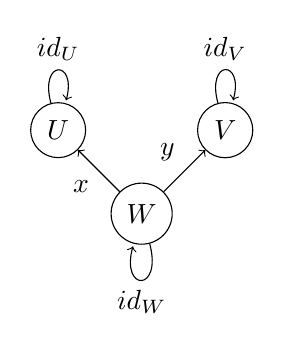
\begin{tikzpicture} [
   ->, node distance=1.5cm, auto, n/.style={circle,draw}
]
   \node (W) [n] {$W$};
   \node (U) [n, above left of=W] {$U$};
   \node (V) [n, above right of=W] {$V$};
   \path (U) edge [loop above] node {$id_U$} (U)
         (V) edge [loop above] node {$id_V$} (V)
         (W) edge node {$x$} (U)
             edge node {$y$} (V)
             edge [loop below] node {$id_W$} (W);
\end{tikzpicture}
\end{example}

\frmrule

\begin{example}
Below shows a category. 
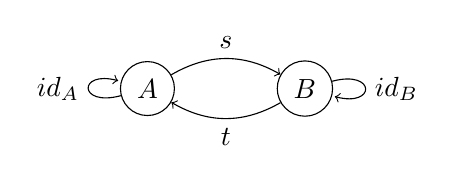
\begin{tikzpicture} [
   ->, node distance=2cm, auto, n/.style={circle,draw}
]
   \node (A) [n] {$A$};
   \node (B) [n, right of=A] {$B$};
   \path (A) edge [bend left] node {$s$} (B)
             edge [loop left] node {$id_A$} (A)
         (B) edge [bend left] node {$t$} (A)
             edge [loop right] node {$id_B$} (B);
\end{tikzpicture}
\end{example}

\frmrule


\begin{example}
Below shows a labelled directed graph.
Complete the following.
\begin{figure}[h]
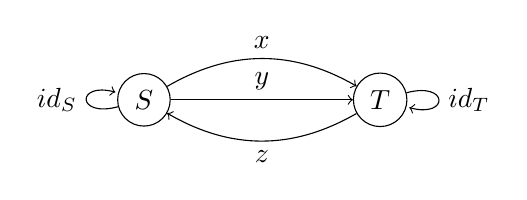
\begin{tikzpicture} [
   ->, node distance=3cm, auto, n/.style={circle,draw}
]
   \node (S) [n] {$S$};
   \node (T) [n, right of=S] {$T$};
   \path (S) edge [bend left] node {$x$} (T)
             edge [loop left] node {$id_S$} (S)
             edge node {$y$} (T) 
         (T) edge [bend left] node {$z$} (S)
             edge [loop right] node {$id_T$} (T);
\end{tikzpicture}
\end{figure}
\end{example}

$$x \star (y \star z) = x \star ... = ....$$
$$(x \star y) \star z = ... \star z = ....$$


\frameans{}
{
$x \star (y \star z) = x \star id_S = \text{undefined}$\\
$(x \star y) \star z = \text{undefined} \star z = \text{undefined}$ 
}


Hence assocativity property fails and so
this graph is \textit{not} a category. 


\frmrule


\begin{example}
Explain why the \textit{outdegree} of every node in a category 
must be at least one? Similarly, why must the \textit{indegree} 
of every node in a category be at least one?
\end{example}


\begin{example}
\end{example}



\section{Introducing Category Theory II}


\highlightdef{Almost \textit{anything} can be viewed as a category} 


Any \textit{partial order relation} $\preccurlyeq \subseteq A \times A$ 
can be transformed to a category where:
\begin{itemize}   
\renewcommand{\labelitemi}{$\Box$}
\item \textbf{Nodes} The nodes of the graph are the elements of the set 
$A$, the same set that $\preccurlyeq$ is defined on.
\item \textbf{Edges} The edges of the category graph are the same 
as the edges in the graph we draw for the partial order relation.  
\item \textbf{Identities} Every partial order relation is \textit{reflexive}. 
The reflexive edges in a partial order graph 
correspond to the identity edges of a category. 
\item \textbf{Composition} 
Every partial order relation is \textit{transitive}.
Having a transitive relationship corresponds to 
composition of edges. 
\end{itemize}


\begin{example}
We define a \textit{less than or equal relation} that 
can order the numbers some between 1 and 25, $A = \{1,6,9,15,22\}$.
Draw the category that corresponds to this partial order relation.
\end{example}

\frmrule

Recall that any kind of \textit{less than relation} 
would not reflexive and so wouldn't be a partial order relation. 


\begin{example}
We define a \textit{divides relation} that 
can order the divisors of 10, $A = \{1,2,4,5,10\}$.
Draw the category that corresponds to this partial order relation.
\end{example}

\frmrule


Any \textit{monoid} $D = \langle A, \square \rangle$ 
can be transformed to a category where:
\begin{itemize}   
\renewcommand{\labelitemi}{$\Box$}
\item \textbf{Nodes} There is exactly one node in the graph.
\item \textbf{Edges} The edges of the graph are the elements of the monoid.
Every edge has the single node as its source node and has the 
single node its target node.
\item \textbf{Identities} We have one node and all the edges start from this 
and come back. However we \textit{uniquely define} the identity $id_D$ to be 
\item \textbf{Composition} 
The composition law is given by the binary operator $\square$. 
\end{itemize}

\frmrule

The operation table for the monoid translates into 
doing composition of edges looping in and out of this single node. 
Here the edges are far more expressive than the node. 
It's important to think of edges \textit{abstractly} rather than 
as perhaps some kind of function (or as pairs of functions). 

Since any monoid can be written as a category, 
we could \textit{redefine} what a monoid is. 

\highlightdef{A \textbf{Monoid} is a category with \textit{one object}}

There is nothing to say that the original definition 
(set grouped with an operator + rules) is more 
fundamental or better than a definition given via category theory. 
They are \textit{equivalent}. 

\frmrule


\begin{example}
$C = (\mathbb{N}, \square)$ is a monoid where the composition law is given by $n \square m = nm$.
Here, $Arr(C)$ is the set of natural numbers. 
\end{example}

\frmrule


\section{Functors}

In mathematics, it is often useful to define the notion of 
a \textit{structure preserving mapping} 
between two instances of a mathematical structure. 
We can acknowledge that there are alike and formally specify 
what properties are the same and what properties differ. 

A \textit{graph homomorphism} is an example 
of a \textit{structure preserving mapping} on a graph. 
Given two graphs, if they are alike enough, 
then we can define a mapping that acknowledges the likeness
in structure.

For graphs,  




\highlightdef{A \textbf{Functor} is a mapping from one category to another ...}
... that preserves the arrows in a particular way. 

the source and target of every arrow, the identity arrow of every node, 
and, the composition law.
